\chapter{SubVis}

Nachfolgend wird das Programm \emph{SubVis} spezifiziert und dessen Architektur vorgestellt.
Außerdem werden die Entwicklungsorganisation, Dokumentation sowie verwendete Bibliotheken dargelegt.

\section{Anforderungen}

\begin{itemize}
 \item Architektur
 \begin{itemize}
 	\item Erweiterbarkeit durch andere Algorithmen mittels Plugins.
 	\item Plugins können eigene GUI-Elemente in dafür vorgesehenen Bereichen zeichnen.
 \end{itemize}
 \item GUI
  \begin{itemize}
 	\item Darstellung des Kontrollnetzes
 	\item Darstellung der Limesfläche
 	\item Rotation des Objektes
 	\item Translation des Objektes
 	\item Skalierung des Objektes
 	\item Beleuchtung der Oberfläche des Netzes, um Glattheit bewerten zu können.
 	\item Edit-Modus: Verschieben eines Punktes anhand seiner Flächennormalen.

 \end{itemize}
 \item Dateiformate / IO
 \begin{itemize}
 	\item OFF-Format und NOFF (mit Farben/Normalen)
 	\item Laden und Speichern von Polygonnetzen
 \end{itemize}
 \item Unterteilungsalgorithmen
 \begin{itemize}
 	\item Catmull-Clark
 	\item Loop
 	\item Doo-Sabin
 	\item Butterfly
 \end{itemize}
 \item Funktionen
 \begin{itemize}
  \item Variable Anzahl von Unterteilungsschritten
  \item Beleuchtungsmodus wählbar
 \end{itemize}
\end{itemize}

\section{Verwendete Tools und Bibliotheken}

\emph{SubVis} greift auf die Bibliotheken Qt, libQGLViewer, Surface\_mesh, OpenGL und Doxygen zurück.
Die verwendeten Versionen sind in \autoref{tab:versionen} ersichtlich.

Die genannten Versionen beziehen sich auf den jetzigen Zustand. 
Während der laufenden Entwicklung wird unter Umständen auf eine jeweils höhere Version aktualisiert.

\begin{table}[h]
\center
\caption{Versionen der Bibliotheken}
\label{tab:versionen}
\begin{tabular}{c|c}
Bibliothek & Version\\
\hline
Qt & 5.4.1\\
libQGLViewer & 2.6.1\\
Surface\_mesh & 1.0\\
OpenGL & 10.1.3-0ubuntu0.4\footnote{Ubuntu Paket mesa-common-dev}\\
Doxygen & 1.8.6\\
\end{tabular}
\end{table}

\section{Architektur}

Es wurde bisher die grundlegende Grob-Architektur festgelegt, welche definiert, welche Komponenten bestehen und wie diese miteinander kommunizieren.
In \autoref{fig:subvis_architektur} ist diese als UML-Komponentendiagramm dargestellt.

Grundsätzlich wird auf eine \ac{MVC} Architektur gesetzt.
Die Model-Komponente soll die Datenstruktur mit dem Polygonnetz beinhalten und Import bzw. Persistenzoperationen anbieten.
Das Delegieren der Ereignisse aus der View-Komponente wird von der Controller-Komponente übernommen. 
Dort sollen auch die entsprechende Signale und Slots definiert werden.
Insbesondere die Editieroperationen werden an die MeshEdit-Komponente übergeben, welche dann die MeshData-Komponente ansteuert.
In der View-Komponente wird die GUI erstellt und gerendert. 
Deren Schnittstelle muss Operationen zum Erweitern der GUI und zum Beeinflussen des Renderings des Hauptfensters bereitstellen.
Auf diese Schnittstelle greifen dann die Plugins zu, die entsprechend eigene GUI-Elemente zeichnen und Plugin-spezifische Renderingmodi anbieten.

\begin{figure}
  \centering
  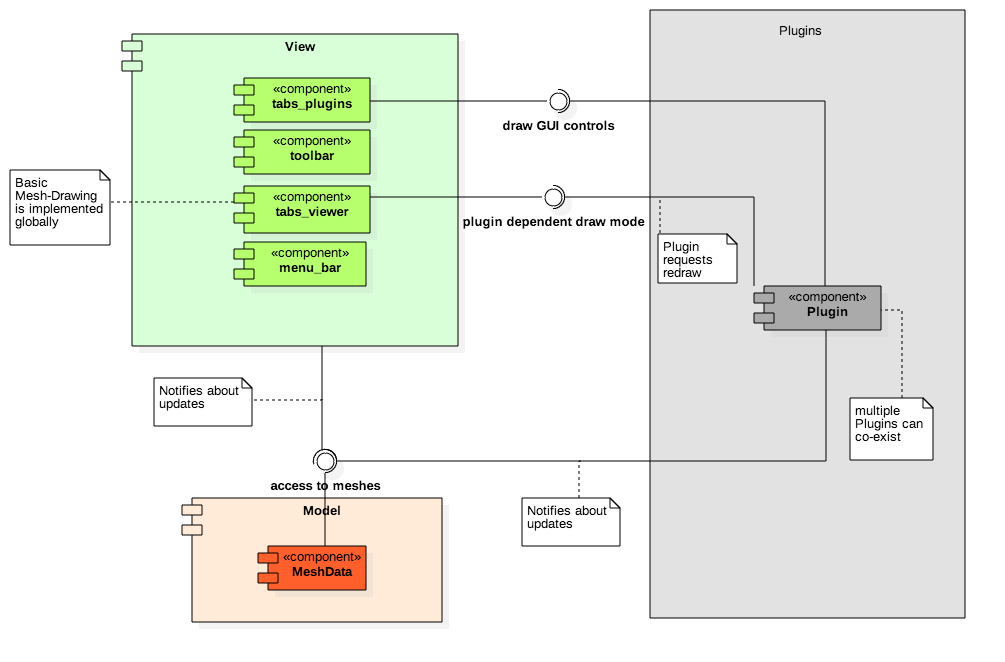
\includegraphics[width=\textwidth]{content/media/subvis_architektur.png}
  \caption{Geplante Architektur von SubVis}
  \label{fig:subvis_architektur}
\end{figure}

\section{Grafische Oberfläche}

Ein erster Entwurf der grafischen Oberfläche ist in \autoref{fig:subvis_gui_mockup} ersichtlich.
Während in der oben angeordneten Toolbar die allgemeinen Bedienelemente angeordnet sind, finden sich in der Plugin-spezifischen Seitenleiste die Einstellungen und weitere Optionen.
Die tatsächlichen GUI-Elemente in der Seitenleiste sind vom Plugin abhängig.

 \begin{figure}[hp]
  \centering
  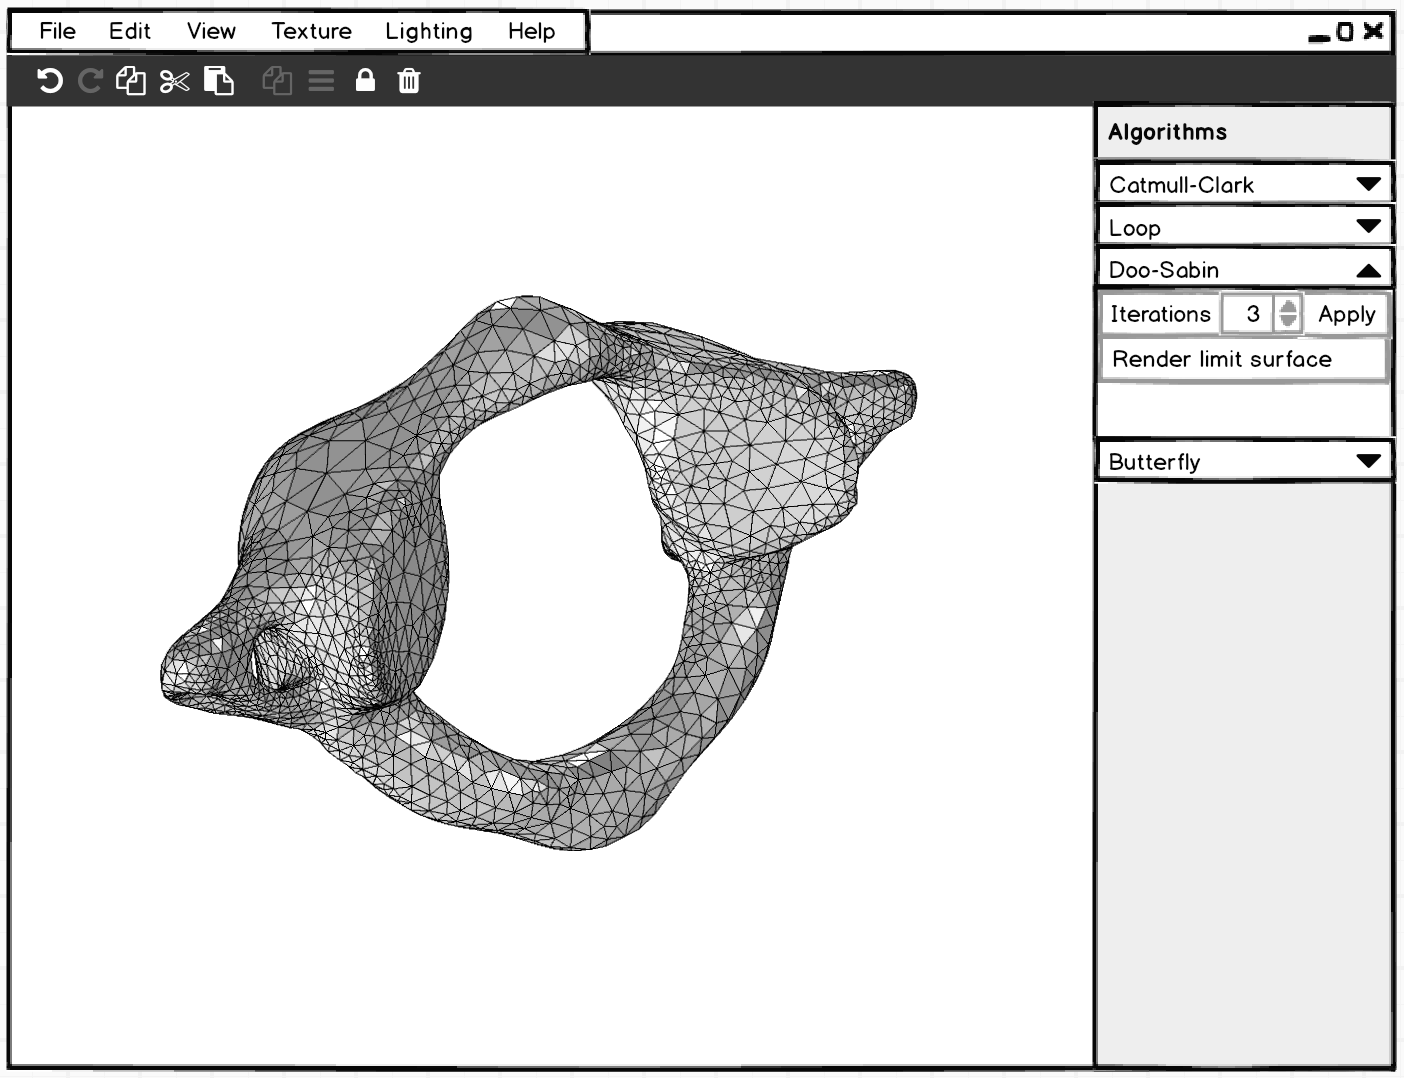
\includegraphics[width=\textwidth]{content/media/subvis_gui_mockup.png}
  \caption{Mögliche grafische Oberfläche von SubVis}
  \label{fig:subvis_gui_mockup}
\end{figure}

\section{Dokumentation}

Die Dokumentation besteht aus diesem Bericht sowie der finalen schriftlichen Ausarbeitung am Ende des 2. Semesters.
Diese Ausarbeitung soll die theoretischen Hintergründe erklären, sowie auf die Entwicklungsprozesse inkl. Vergleich und Entscheidungen für spezifische Technologien eingehen.
Ziel ist es, dem Leser eine Top-Down-Ansicht auf das Projekt zu verschaffen.
Es wird bewusst auf eine detaillierte Quellcodedokumentation in der Ausarbeitung verzichtet, um die Dokumentation nahe am Quellcode und aktuell zu halten.

Durch Quellcodedokumentierung sollen Entwickler befähigt werden schnell in das Projekt einsteigen zu können und das Programm weiter zu entwickeln bzw. durch Plugins zu erweitern.
Insbesondere bei den Plugins soll ein kurzes Tutorial erstellt werden, welches an die Plugin-Entwicklung heranführt. 
Des Weiteren soll ein kleines, gut dokumentiertes Plugin entstehen, um den prinzipiellen Aufbau zu veranschaulichen.
Wenn zu viel dokumentiert wird, veraltet diese schneller.
Deswegen soll \emph{sinnvoll} und \emph{angemessen} dokumentiert werden.
Dies bedeutet öffentliche APIs, wenn notwendig, detailliert und ausführlich zu dokumentieren und selbsterklärende Funktionen etc. nicht unnötig zu dokumentieren.
Grundsätzlich soll der Quellcode selbst schon als Dokumentation dienen können.
Zusätzlich finden sich beim Quellcode README-Dateien, die genaue Details über die verwendeten Funktionen, Build-Anleitungen und die Projektstruktur erläutern.

\section{Entwicklung}

Um eine gemeinsame Entwicklungsumgebung zu schaffen, wurden gewisse Bibliotheken, Tools und Plattformen spezifiziert.
Dies betrifft einerseits die Bibliotheken und Tools aus \autoref{tab:versionen}.
Andererseits auch das Betriebssystem, Versionsverwaltung, IDE und Programmiersprachenstandard.

Als Betriebssystem wird Ubuntu 14.04 LTS verwendet. 
Zum Projektabschluss wird jedoch eine plattformunabhängige Anwendung angestrebt.
Die Sprachfeatures von C++ sollen maximal dem C++11 Standard entsprechen.
Als Versionsverwaltung wird Git in Verbindung mit dem Git-Server des IOS an der HTWG eingesetzt. 

Die Entwicklung findet auf dem \emph{develop}-Branch und eventuellen  Feature-Branches statt.
Dabei sollte ein Branch pro Feature erstellt werden und erst dann in den develop-Branch gemergt werden, wenn das Feature funktioniert.
Als IDE wird der vorgestellte Qt Creator verwendet.

Das Projekt teilt sich in zwei Verzeichnisse auf: \emph{SubVis} und \emph{dev-doc}.
\emph{SubVis} enthält die gleichlautende Anwendung als Qt-Projekt und unterteilt sich noch in die Ordner \emph{app}, \emph{lib} und \emph{objs}.
\emph{app} enthält die Anwendungsteile die selbst entwickelt werden,
\emph{lib} die Drittherstellerbibliotheken und \emph{objs} 3D-Modelle zum Testen.
\emph{dev-doc} dient der weiterführenden Dokumentation.
Das Verzeichnis enthält z. B. Diagramme, diesen Bericht und andere hilfreiche Dokumente zur Entwicklung.
































